\documentclass[10pt]{article}

\usepackage{amsmath}
\usepackage{graphicx}
\usepackage{float}
\restylefloat{table}
\usepackage{hyperref} 
\usepackage{animate}
\usepackage{subfig}
\setcounter{tocdepth}{4}
\setcounter{secnumdepth}{4}


\title{Understanding Opinion Dynamics in Social Networks\\
		Background and Progress Report}
\author{John Freeman}

\begin{document}
\maketitle
\pagebreak
\tableofcontents
\pagebreak

\section{Background} 

The world has always been composed of networks. From the simplest intracellular protein networks to the most complex food webs and ecosystems, almost all real-world phenomena are results of smaller networks or a components of larger ones. While these real-world networks have been and continue to be difficult to study due to the difficulty of collecting good data, the advent of the information age has led to the emergence of new classes of human designed and built networks that are inherently easier to study. \\

Today, we have a wealth of data available to us about many networks in the world, ranging from rail networks to phone connections to the focus of this project: social networks. While social networks are a broad category, including such different phenomena as modern social media websites and interactions within pods of dolphins, many of the underlying behaviors of the networks remains remarkably constant. We will however be focusing on online social networks as they have the most data available, and as a consequence are the most well studied. \\

\subsection{Networks and Models} 

We can describe a social network as a simple undirected graph $G$, composed of some edges $E$ and some vertices or nodes $V$. In general, the vertices of a social network correspond to the individuals or entities that inhabit it. The edges have a bit more variance in what they can represent, but in general and in our case denote a "friend" or "follow" relation, a trivial example being an edge exists between two people $v1$ and $v2$ if they are friends in the given network. \\

Many models have been put forward to simulate the behavior we see in real-world networks, social or otherwise. We will be combining three models in this paper to try to build a comprehensive model of a social network: the Apt-Markakis model of product adoption, the Schelling model of self-segregation, and the Barabási–Albert model of scale-freeness. Each of these three models simulates a different aspect of social networks we hope to capture: Apt-Markakis handling opinion spread, Schelling handling group formation, and Barabási–Albert keeping the network scale-free. \\

The Apt-Markakis model \cite{apt2011diffusion} was designed to model the diffusion of products across a social network. In the simplest case, each node is initialized to have either adopted a product, or a threshold at which it will adopt one. The model then continuously checks nodes that have not adopted products to see if the fraction of its neighbors that have adopted a given product exceeds the node's threshold. If a node's threshold is met, it adopts the most common product of its neighbors. Apt and Markakis go on to show numerous results of computational complexity of various problems on their model, but the aspect of it we take advantage of in this project is its ability to easily model product, or in our case opinion, diffusion across a network. \\

A natural synergy with the Apt-Markakis model is Schelling's model of self-segregation \cite{schelling1971dynamic}. In Schelling's model, nodes evaluate whether they are satisfied in their location or not by checking how many dissimilar neighbors they have. Should a node be dissatisfied, it will move to a neighborhood that is more similar to itself, again according to dissimilarity thresholds. Schelling's model has been extensively studied and has been shown to accurately characterize many more real-world behaviors than those put forwards in his paper. It is especially useful to us as it provides a mechanism to make our model dynamic, with connections being made and broken according to node opinions and tolerances. \\

A common if not ubiquitous characteristic of real-world networks is scale-freeness, a term used to describe graphs with log-linear degree distributions. Many models have been put forwards to create networks with this property, but arguably the most popular is the Barabási–Albert model \cite{barabasi1999emergence}. In the model, we start with an initial graph and continuously add nodes to it. At each addition, we calculate the probability an edge exists between it and a given node in the graph by the proportion of its degree to the total degree of the graph. This simulates a "rich get richer" system where nodes with higher degree will have their degrees increase faster than those with lower degree, which in turn yields a scale-free network. \\

The three of these models put together should allow us to build a composite model that simulates some essential features common to real-world networks: formation of communities based on shared ideas, a log-linear degree distribution, and hopefully as a result of the aforementioned community formation and scale-freeness: small world structure, another common feature of social networks. \\

\subsection{Machine Learning on Graphs}

Traditionally, graph theoretic problems have been addressed through mathematical and computer scientific approaches, with complexity classes being extensively studied and approximation algorithms being created to deal with the NP-completeness that is pervasive in graph-based problems. While such approaches are generally successful, modern data-driven methodologies have become increasingly common in the analysis of graphs, especially on large real-world datasets. \\

Machine learning type algorithms have arrived relatively late to graph problems, in a large part due to the dissimilarity of the data to other approaches. Most algorithms rely on input vectors of numerical data and have few ways of efficiently representing topological information of the graphs themselves, often forcing them to resort to using node attributes augmented by simple human made features. Worse still is the case of unattributed nodes where the topology of the network is all that can be learned from, where algorithms are reduced to considering adjacency information alone. While attribute information is no doubt useful, the topology of the graph often contains more useful information, especially for graph theoretic problems. \\ 

A common way of applying machine learning techniques to graphs is to create a graph embedding, that is, converting the graph into a vector space. Many techniques exist for this: initially spectral methods based off adjacency matrices and other information, and later based off random walks and eventually deep learning methods on the graph itself. The key in graph embeddings is to find a representation vector for a given node such that the structural and attribute properties of the graph are preserved in the embedding vector space. \\

The problem of graph embeddings has been extensively studied in the case of static, unchanging graphs \cite{goyal2018graph}. In our project however, we hope to capture information about opinion dynamics, which is as the name suggests a dynamic process. As such, we need an embedding method that will work for graphs that change over time. This is a new research area, although there has been work in online spectral methods 
\cite{li2017attributed}, as well as dynamic autoencoders \cite{goyal2018dyngem}, among others. We hope to make use of autoencoders as well as random walkers for a method that we hope will combine the best aspects of both while being fully online. \\

\subsubsection{Autoencoders}

An autoencoder is a class of neural network designed around finding an encoding for a given input. Generally symmetric about an embedding layer significantly smaller than the input dimension, an autoencoder tries to optimize similarity of the reconstructed input to the true input to find a low dimensional encoding of the input from which all the inputs characteristics can be reconstructed. While numerous variations exist, most architectures follow this pattern with no more than a few changes. Autoencoders have recently become more popular with finding embeddings for graphs and are generally used to encode first and second order proximities of nodes. Thanks to the ease with which neural networks can dynamically self-scale themselves to larger inputs, autoencoders and are one of the easiest methods to generalize to dynamic graphs. \\

\subsubsection{Convolution on Graphs}

Arguably the most significant standard operation in neural networks is the convolution operator. Originally conceived from signal analysis, the convolution operator allows a network to consider the local context of a data point, learning a filter of the data and its neighbors. The convolution operator is easy to use for images, where the neighbors of a pixel always have the same shape as an image has a standard structure. On graphs however, we face more issues stemming from the varying degrees of its nodes. \\

Many ways to generalize convolution to graphs have been proposed \cite{wu2019comprehensive}, in the simplest cases based on $out = \sigma (AXW)$, where $\sigma$ is an arbitrary activation function, $A$ is the graph's adjacency matrix, $X$ is the graph's node-wise attribute matrix, and $W$ is a learnable weight matrix. Many other generalizations exist, ranging from normalized versions of the equation above to variants using spectral information to kernel models featuring a myriad of distributions. \\

Luckily for us, the PyTorch Geometric \cite{Fey/Lenssen/2019} has recently been released and gained significant popularity. PyG implements a wide variety of graph operations while seamlessly interfacing with PyTorch and achieving execution times we couldn't hope to match through heavy integration with CUDA. We anticipate PyG will be integral to the success of our project, as graph convolution will yield significant speedup compared to existing models and should also yield significant increases in model quality. \\

\subsubsection{Random Walks and Ant Colonies}

Arguably the most successful method in graph embeddings, and the one that catalyzed the field as a whole, is random walks. Drawing inspiration from language models, random walk-based methods such as DeepWalk \cite{perozzi2014deepwalk} run a random walk at a given node and run it against a typical skip-gram model or other language embedding framework. The random walk yields a sequence of nodes that appear in the "context" of a given node, closely mirroring words appearing in the context of another in human language. This similarity can be exploited by applying well-studied natural language word embedding algorithms to the problem of graphs. DeepWalk was able to achieve massive improvements over existing spectral and other human-designed feature based methods, and serves as an inspiration for what we intend to use for our  model. \\

Another research area that had decent amount of success in the community detection domain was that of artificial ant colony algorithms \cite{bertelle2006organization, zhou2015ant}. In these models, the network has numerous random walkers traversing it, but with some extra heuristics added to the walkers to simulate the behavior of ants. After traversing an edge, the random walker deposits pheromones on it, which in turn increases the probability of another walker taking that edge. As time passes, pheromone levels decrease on an edge according to some heuristic, to help promote exploration. A common method of community detection for example involves the ants probabilistically depositing the label of some previous node they visited on their current node, with the most common label at the end of the algorithm being their community assignment. \\

With some minor modifications, we believe that the ant colony methods provide us with a framework to generalize random-walk based methods to dynamic graphs. The ants can be run in parallel with network updates, continuously updating the random walk associated with a given node. Since our model will follow a power-law degree distribution, the nodes with highest degrees will be most traversed and likewise the most updated. Likewise, we believe the dynamic autoencoders could be augmented by graph convolutions to significantly increase the power of existing dynamic models. \\

\subsection{Related Work}

As referenced above, our main inspirations are drawn from existing systems that we hope to extend to the dynamic case. Deepwalk, ant colonies, and other random walk based algorithms provided good baselines but were limited by not being able to capture the global structure of graphs and not being easily able to handle structure changes. Neural network architectures perform well on spectral and adjacency information and can be extended to the dynamic case, but still lack the whole context of the graph. \\

Graph convolutional neural networks solve most of the above problems, at the cost of complexity: they need to operate on the entire graph at once rather than individual nodes. They are however able to achieve significant performance increases over the local methods, and while they have not yet been tested significantly in dynamic graphs, we believe that they should be able to handle them as standard convolutions are ubiquitous for speech processing and other time-series data. \\

A system similar to the one we propose has already been implemented by Ying et al \cite{ying2018graph}, where they combine both random walks and graph convolutions to embed huge graphs. Although we will not have access to the computational power they had, we hope to build off it by applying the framework to dynamic graphs, as well as exploring several novel graph problems with it once complete. \\

\pagebreak

\section{Project Proposal}

In social networks, opinions are everywhere. They both influence and are influenced by the networks they exist in, but in all cases they are dynamic. Building off existing research, we intend to build a model that can simulate dynamic opinion spread in networks, and a system to embed those networks in real time. Should time allow, we then intend to study several graph-theoretic problems on our model through our embeddings. \\

We will build a model that combines the Apt-Markakis, Schelling, and Barabási–Albert models into one framework that will allow us to have an easy to use toy model to build an embedding system off of, and hopefully to explore emergent properties arising from the combination of those models. We want to build our own network instead of focusing on precompiled datasets as it will allow easier exploration of various network sizes and structures within an easy to use framework. \\

The embedding system will be either convolution or random walk based, or some combination thereof. In the former, we will pursue a standard autoencoder architecture making use of graph convolutions with some experimentation in architecture and methods to generalize to the dynamic case. In the latter we will have artificial ants continuously traversing the network in parallel with its evolution. After each network update, we will check which old edges were broken and will remove nodes from the ants memory prior to their traversing that edge. To generate the actual embeddings, we will feed the ant's walk information on a node level through an autoencoder, or some other similar neural network, to generate embedding vectors for each node. We will compare these embeddings against existing methods to verify their effectiveness, and then use them to study various graph-theoretic problems related to opinion diffusion on our network, and in the real world. \\

\section{Objectives}

\subsection{Critcal}
\begin{itemize}
\item The model must be able to simulate a dynamic, self-organizing social network that exhibits known properties of scale-freeness and community formation
\begin{itemize}
\item \textit{Feasible}. A proof of concept model has already been created that appears to satisfy the objectives. It has not been rigorously verified yet, but based on what we have so far we don't anticipate issues with this goal. 
\item \textit{Verification Plan}. As the model is not the focal point of the project, verification will be relatively light. That being said, it is critical for our model to represent known properties of real-world networks. Specifically we want it to create a small-world network that is scale-free, as those two properties are known to arise in the vast majority of real world networks. Luckily, both these properties will be easy to verify: 
\begin{itemize}
\item \textit{Scale-Freeness}. A network is scale-free if its degree distribution is asymptotically log-linear, or equivalently if its degree distribution follows a power law. Either of these properties can be verified trivially by plotting the degree distribution and fitting a curve. 
\item \textit{Small-Worldness}. Small-worldness is another property that has been studied extensively. While it has been shown that all scale-free networks are also small-worlds \cite{cohen2003scale}, we will still verify this by the $\omega$ metric proposed by Telesford \cite{telesford2011ubiquity}. 
\end{itemize}
\item \textit{Contingency Plan}. Should we fail to construct a model, we will turn to standard datasets for dynamic networks from Stanford's SNAP collection \cite{snapnets}. As we plan to use these datsets for real world exploration anyways, being forced to use them will not be a significant loss. 
\end{itemize} 
\item We must be able to construct a system to embed nodes in our network into vectors, with online updates as the model runs
\begin{itemize}
\item \textit{Probably Feasible} - We have identified several paradigms we can approach this problem from, described in more detail below. While dynamic graph embedding is a hard problem, it is a new research field and as such there are many angles we are free to explore. 
\item \textit{Verification Plan} There are several metrics and best practices available for verifying the accuracy of node embeddings, one of the most common being label prediction. Given a labelled dataset, we attempt to predict the label on a held out test set and compare accuracy to existing methods. Numerous other metrics exist and we will attempt to follow standard comparison practices as well as we can. 
\item \textit{Contingency Plan} - This goal is essential to completion of the project as it features the most novel and significant work. Should we fail to complete it however, there are existing embedding frameworks we can use to study community formation behaviors in models and datasets. 
\end{itemize}
\end{itemize}

\subsection{Planned}
\begin{itemize}
\item We would like our model to emergently exhibit known real-world properties of social networks, including small-world characteristics, a dense core and clustered fringe, and a power-law group distribution.
\begin{itemize}
\item \textit{Difficult} - Online social networks have a multitude of complex behaviors underlying them. Even getting the simple model from above has a high time complexity to simulate and adding more properties could further slow it down. That being said, if time allows we plan to look into optimizations and methods to get these features. 
\item \textit{Verification Plan} We will follow the quantitative measures described by Mislove et al \cite{mislove2007measurement}, including sub logarithmic increase in path length when removing core nodes for checking dense cores, and clustering coefficients for checking power-law group distributions. 
\item \textit{Contingency Plan} - This goal is not as important as the embedding system, but as we use the model to develop the embedding system in the first place, we want it to be as real world as possible. That being said, if the other model goals are met we will still be able to move on with the rest of the project. 
\end{itemize}
\item We would like our embedding system to compare favorably to other existing systems, whether in time or general performance. 
\begin{itemize}
\item \textit{Difficult} - Dynamic node embedding is a new research field for good reason: it's difficult. That being said, we do feel that our method will combine the best features of autoencoders and random walk based methods while still functioning on a dynamic graph, so we hope to at least be able to match existing methods like Li et al's DANE and dynamic autoencoders. 
\item \textit{Verification Plan} We will largely follow the same verification plan as we did for our whole model, but run those same metrics through other embedding models to compare results. We will measure task performance as well as time taken, and hope to have at least comparable performance in one or both of those spaces.  
\item \textit{Contingency Plan} - Failure in this goal could mean many things, ranging from the chosen embedding approach simply doesn't work, to the implementation being wrong. In any event, this is more of a goal to work towards: progressively improving the algorithm and making changes as necessary. We don't anticipate that we will be able to significantly surpass existing methods, but we do believe we believe with sufficient work we can at least get close. 
\end{itemize}

\end{itemize}

\subsection{Reach}
\begin{itemize}
\item Research and study applications of our embedding system to a given graph theoretic problem, ie influence maximization, clique detection, and so on. 
\begin{itemize}
\item \textit{Probably Feasible} This goal would be more to demonstrate the effectiveness of our embedding system. We would select a graph problem of our choosing and then use the embeddings to evaluate a solution to that, then compare it to the graph algorithm equivalent solution. Assuming our embedding works, this should be doable, but time consuming.
\end{itemize}
\end{itemize}

\pagebreak

\section{Model Design}

The model will be a combination of the of Apt-Markakis, Schelling, and Barabási–Albert models. The only major aspect of the models we intend to change is to make the products of the Apt-Markakis section be continuous-valued vectors instead of categories. We believe that this change will allow for more dynamical systems and better model real-world data. 

\begin{itemize}
\item The model will start in an initial state with some nodes and edges
\item Each node will be initialized to have a random continuous-valued vector as its product, or with a threshold as in a standard Apt-Markakis model. It will also have a schelling threshold, which will describe how far another node needs to be from itself to be considered different
\item At each time step of model evolution, there will be three actions: a network update step, an Apt-Markakis step and a Schelling Step
\begin{itemize}
\item In the network update step, we base an update on the Barabási–Albert model, adding a random amount of new nodes with connections proportional to the degree of nodes of the existing network
\item In the Apt-Markakis step, each node (or some node at random) that has its threshold met for some index of its opinion vector will adopt the median or average opinion of its neighbors, with some optional gaussian noise added in
\item In the Schelling step, each node that is dissatisfied, where dissatisfaction is determined by the distance between its opinion average or median opinion of its neighbors, will be able to adjust its edges until it is satisfied by making/breaking connections. The nodes it considers to make or break connections will be randomly sampled according to a probability distribution built off of existing node degrees, as well as proximity to the dissatisfied node
\end{itemize}
\item The embedding system will run after the network finishes its update cycle for a given time step 
\end{itemize}

This model would allow for numerous possible frames to be explored, including starting from a network with communities and making new ones form off it through addition of nodes, or starting from a completely random network and allowing the system to self-organize. \\



\pagebreak

\section{Dynamic Node Embedding System Design}

We propose to follow one of two paradigms for our model: one based on random walkers and one based on graph convolutions. We intend to implement trivial models of each and then either further refine the one that seems more promising, or combine the two for a fully developed final model. \\

\subsection{Random Walker Proposal}

The first proposal for the embedding system is to build a novel system for dynamic graphs combining random walkers with autoencoders. Random walkers will continuously traverse our graph, updating nodes as they pass them with other nodes from the walkers memory. After each complete network update cycle, the autoencoder will run through a training cycle with the updated walker data. We also hold open the possibility of using some other language model instead of an autoencoder, and augmenting node data with additional information, such as first order proximity or other features. 
\begin{itemize}
\item Each node will have a list $related$, initialized to contain its neighbors, which will be filled up as the walkers traverse the graph
\item In parallel with network updates, walkers will move about the graph in step with transition probabilities corresponding to various heuristics, ie pheremone levels on edges, neighborhood information, neighbor degree, and so on
\item Each time an ant visits a new node, it will sample at random some sequence of the prior nodes it has visited and add them to the new node's list according to some heuristic. After each step, the pheremone level on the traversed edge will be increased to promote exploration
\item After each network update cycle, the nodes' lists will be pushed through an autoencoder to generate embedding vectors. If the network size was increased, we need simply run a Net2WiderNet \cite{chen2015net2net} call on our autoencoder to account for the new nodes 
\end{itemize} 

\subsection{Convolutional Autoencoder Proposal}

A second paradigm we would like to explore is that of graph convolution. As described previously, convolution is a powerful tool for machine learning on graphs, and one that has yet to be significantly explored in the context of dynamic graphs. This model would also have the advantage of having fewer moving parts, so to speak, in that it would would not have to deal with synchronization and node traversal rates and other issues with the random walkers.  \\

\begin{itemize}
\item The model would be again an autoencoder architecture, but this time utilizing graph convolutions instead of linear layers
\item The model would be run after each network update, again utilizing Net2Net to change the model's dimensions. This would however require some extra work, as Net2Net does not appear to have been tested on graph convolutions
\item There would be many possibilities for the model architecture, as there have been many implementations and descriptions of graph convolution. We would be free to test existing models or to design one of our own, and would determine the best path after sufficient testing
\end{itemize}

\pagebreak

\section{Exploring Graph Problems}

We plan to explore numerous problems using our generated embeddings, generally falling into three types: those we will use to verify the efficacy of our embedding system, those we will use to improve it, and those we plan to solve using it. 

\begin{itemize}
\item The obvious problem to solve given our model is opinion clustering. Each node will have a value associated with the Apt-Markakis portion of the model, and if our embedding works we would expect nodes with similar products to be close to each other in our vector space even if the opinion isn't considered in our embedding
\item A similar problem is node proximity, verifying that nodes close to each other in a graph are close to each other in the vector space, or similarly that distance in the vector space will be proportional to shortest path distance in the graph
\item A more challenging problem we would like to solve is building a system or model to predict trajectories of nodes in the vector space, effectively what direction we expect them to move in as time passes in the dynamic network, thus giving insights on the dynamics of the system as a whole
\item Another problem would be community detection, an area were we could perform more novel research. Most approaches to community detection through machine learning methods involve applying traditional clustering algorithms on the embeddings which carries all the intrinsic disadvantages of using models on models. Recently however there has been research on training autoencoders side by side with a clustering network \cite{xie2016unsupervised, zhang2019deep}, a technique we believe could easily be adapted to graph models. Should our embeddings be accurate, we believe that such deep clustering frameworks should easily identify known communities in graphs in step with the encoding system itself
\item There are numerous ways we could improve our model, largely based around having it encode extra information, such as shortest path length, clique membership, node influence, or other properties like bridge membership
\item One final problem we can consider is finding ways to optimally segment our graph for use in graph convolutional networks. An unfortunate limitation of such networks is that they can generally only operate on an entire graph, which becomes an issue when dealing with massive datasets. Using our model, we could study methods for partitioning our graph into components that yield good embeddings when processed in mini-batches as opposed to a full-dataset batch \\
\end{itemize}

\pagebreak

\section{Schedule}

\textbf{May}
\begin{itemize}
\item Week of May 6 - Begin background reading
\item Week of May 13 - Continue background reading, begin implementation of proof of concept model, start on progress report
\item Week of May 20 - Continue background reading, complete proof of concept model
\item Week of May 27 - Build proof of concept embedding system
\end{itemize}
\textbf{June}
\begin{itemize}
\item Week of June 3 - Finalize and submit progress report, work on stopping the model from excessively clustering
\item Week of June 10 - Finalize model by refactoring, optimizing, and fixing clustering issue
\item Week of June 17 - Build a convolutional embedding system
\item Week of June 24 - Build a random-walker embedding system
\end{itemize}
\textbf{July}
\begin{itemize}
\item Week of July 1 - Finish the random-walker system, start working to combine the two
\item Week of July 8 - Finalize the entire embedding system
\item Week of July 15 - Compare embeddings to known models on standard datasets
\item Week of July 22 - Finish embedding system comparisons, choose some reach goals that seem most achievable given state of the model
\item Week of July 29 - Work on reach goals
\end{itemize}
\textbf{August}
\begin{itemize}
\item Week of August 5 - Finish up reach goals
\item Week of August 12 - Slack time
\item Week of August 19 - Start on final report
\item Week of August 26 - Work on final report
\end{itemize}
\textbf{September}
\begin{itemize}
\item Week of September 2 - Finalize report, build slide deck, prepare for presentation
\item Week of September 9 - Prepare for presentation, final presentation
\end{itemize}

\pagebreak

\section{Progress}

Progress so far has been limited to building a proof of concept model, planning, experimentation, and background reading. So far we have not hit any major obstacles and believe that we will be able to follow the above schedule without too many roadblocks. \\

We have managed to succesfully implement a proof of concept model as described in our plan, and it seems to behave as expected. In the case of scalar products the model can easily scale to around 2500 nodes, but in the vector case we see significant slowdown limiting us to around 500 even in the case with only two values per node. That being said, all emergent behavior we have been able to demonstrate with higher length vectors we have also been able to demonstrate with scalars, and based on some cursory checks scalar networks appear to better exhibit small-world properties. As our model is currently working, the main thing left to do on it is to try to make some optimizations as well as refactor the code, which currently resides in a classless iPython Notebook. We also need to run some verifications as described in the objectives section, which will be time consuming but not difficult.  \\

Our model has several parameters, the three most important ones being iteration length, vector length, and initial product adoption. The iteration length is as one would expect the amount of time steps the model goes through. While this of course allows the Schelling and Apt-Markakis steps to progress, it also allows nodes to be added by the Barabási–Albert component. In our implementation we add a node with a variable probability, currently set to 0.6, and initialize the network to have 25 nodes. As such, after $t$ time steps, we would expect our network to have $0.6t + 25$ nodes. The vector length corresponds to the amount of opinions each node has, which tends to promote sparse graphs the higher it goes. Lastly, the initial adoption parameter is what percent of nodes start with an opinion. We have found that increasing this helps promote community formation and as such kept it fixed at 0.7 for all runs. \\

\begin{center}
\begin{minipage}{0.48\linewidth}
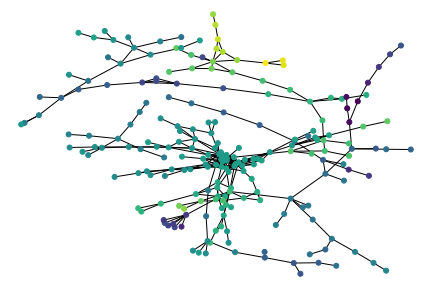
\includegraphics[width=\linewidth]{images/final1558604791.png}
\captionof{figure}{300 iterations, vector length 2, 70\% adopted products}
\end{minipage}%
\hfill
\begin{minipage}{0.49\linewidth}
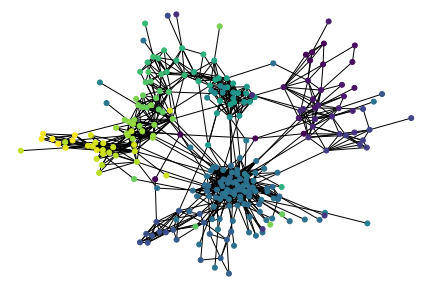
\includegraphics[width=\linewidth]{images/final1558604650.png}
\captionof{figure}{500 iterations, vector length 1, 70\% adopted products}
\end{minipage}
\end{center}
\begin{center}
\begin{minipage}{0.49\linewidth}
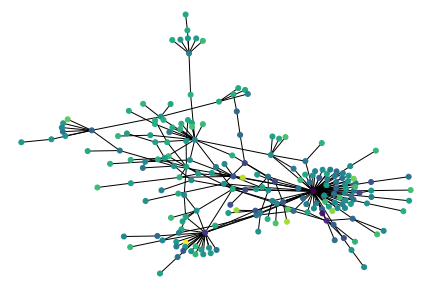
\includegraphics[width=\linewidth]{images/final1558607182.png}
\captionof{figure}{300 iterations, vector length 15, 70\% adopted products}
\end{minipage}
\hfill
\begin{minipage}{0.49\linewidth}
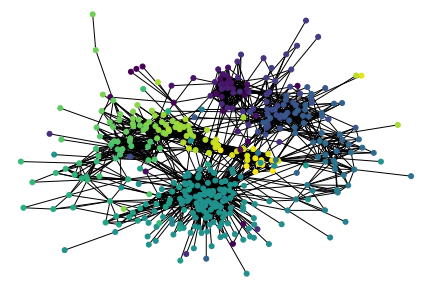
\includegraphics[width=\linewidth]{images/final1558607425}
\captionof{figure}{750 iterations, vector length 1, 70\% adopted products}
\end{minipage}
\end{center}

We have also been working to construct an autoencoder for static graphs, and have thus far implemented a simple model that can reproduce many standard results. It should serve as a platform to build the dynamic version off of with some modifications, and thus far we do not anticipate any issues on that part of the project. We have also begun testing various convolutional operators, after spending significantly more time than planned getting CUDA and PyG up and running. Again however, after the initial installation issues results are promising and we anticipate no further roadblocks. \\

Our model seems to be performing well, witnessed by the figures below. In figures 8 and 9 we see a comparison of K-Means clustering on the embeddings and a community detection algorithm on the graph itself. While they are not a perfect match, the similarity between the two indicates the embeddings capture the structure of the graph well. In figure 9, we see a visualization of some trained 2d embeddings compared to the graph they were generated against. The model never saw the Apt-Markakis opinions but in the embedding space they are clearly seperated, indicating both that the graph model works as intended, and that the embedding system adequately captures its structure. \\

\begin{center}
\begin{minipage}{0.48\linewidth}
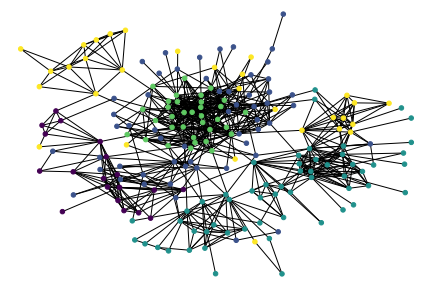
\includegraphics[width=\linewidth]{images/kmeans.png}
\captionof{figure}{K-Means Clustering on Embeddings}
\end{minipage}%
\hfill
\begin{minipage}{0.49\linewidth}
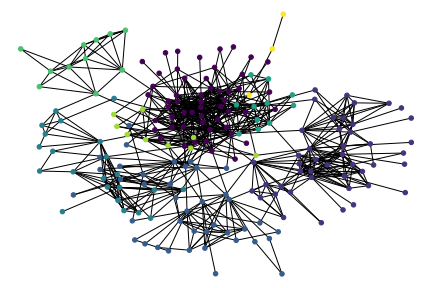
\includegraphics[width=\linewidth]{images/communities.png}
\captionof{figure}{Greedy Community Detection Algorithm}
\end{minipage}
\end{center}

\begin{center}
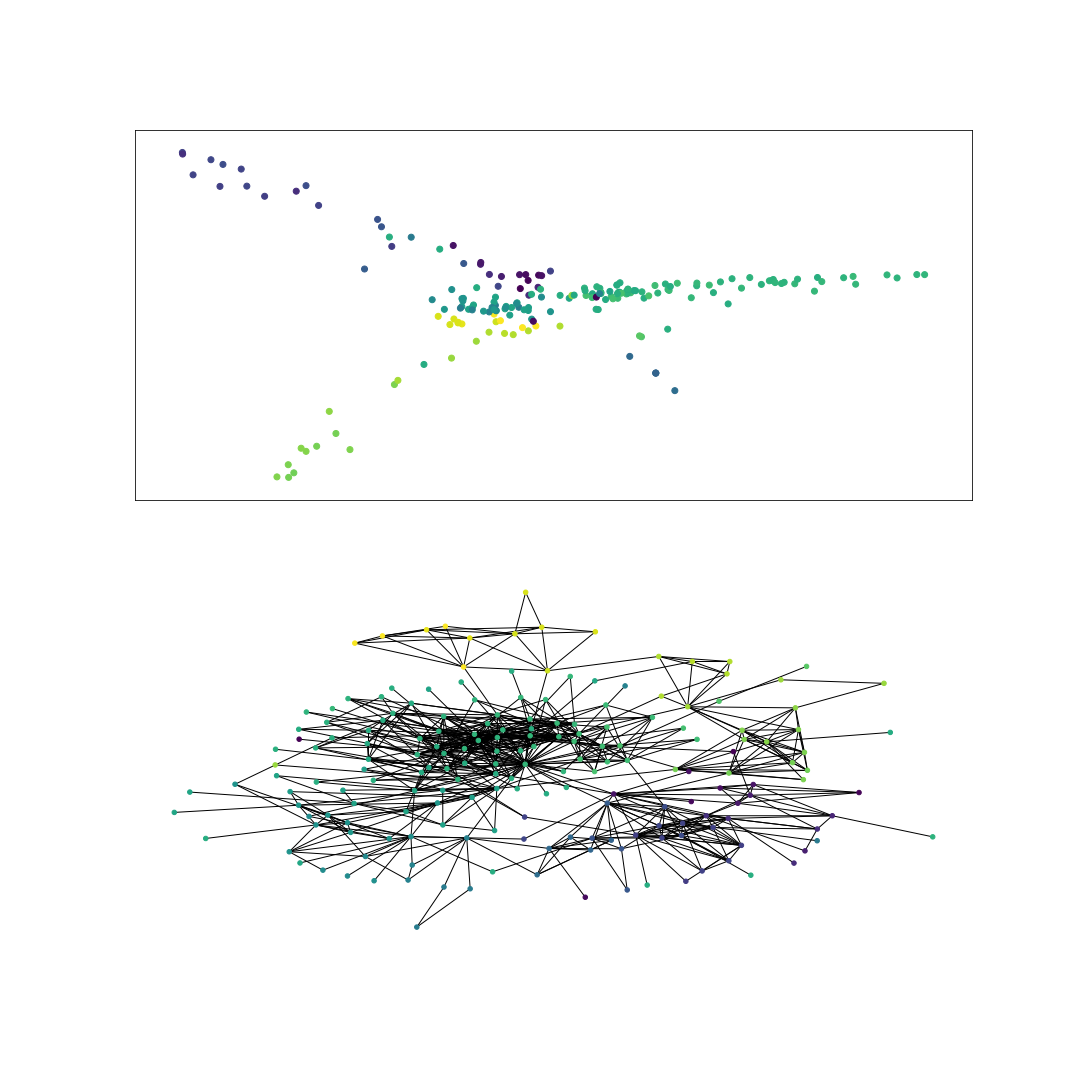
\includegraphics[width=\linewidth]{images/embed_anim/72}
\captionof{figure}{2d embedding generated from a time series of graphs}
\end{center}

\pagebreak

\addcontentsline{toc}{section}{References}

\bibliographystyle{unsrt}
\bibliography{bibliography} 

\end{document}